\documentclass[12pt,letterpaper,titlepage]{article}

\usepackage{fontspec}
\defaultfontfeatures{Mapping=tex-text}
\usepackage{xunicode}
\usepackage{xltxtra}
\usepackage{amsmath}
\usepackage{pdfpages}
\usepackage{amsfonts}
\usepackage{bbold}
\usepackage{amssymb}
\setcounter{secnumdepth}{0}
\usepackage{nameref}
\usepackage{enumitem}
\usepackage{environ}
\usepackage{pgfplots}
\usepackage{listings}

\showboxdepth=\maxdimen
\showboxbreadth=\maxdimen


\usepackage{paracol}
\usepackage{wrapfig}
\globalcounter{table}
\globalcounter{figure}
\usepackage{graphicx}
\usepackage[left=1in,right=1in,top=1in,bottom=1in]{geometry}
\graphicspath{{img/}}

\author{Jacob Abel}
\title{	Design \& Simulate 16
	\\\large ECE2204 CRN:82929
}

\setlength{\parskip}{0.5em}

\begin{document}
\maketitle
\begin{raggedright}
\columnratio{0.6}
\begin{paracol}{2}
\switchcolumn
\begin{center}
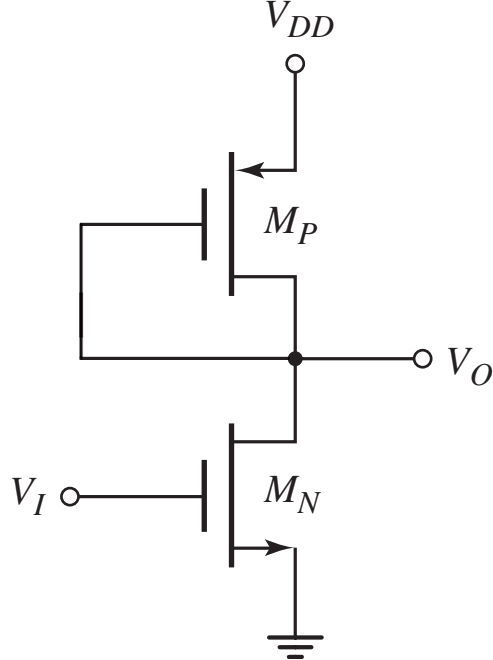
\includegraphics[width=\textwidth, height=17\baselineskip, keepaspectratio=true]{ds1}
\end{center}
\switchcolumn
\section{Problem 16.3-9.a.1: } 
\subsection{Design}

For the circuit below, find $V_{It}$, the modes of operation of the MOSFETs, $V_O$, $I_D$, and the static power. Assume $V_{TP} = -1V$, $V_{TN} = 1V$, $K_p = 10\mu A/V^2$, $K_n = 50\mu A/V^2$, $\lambda = 0$, $V_{DD} = 5V$, and $V_I = 5V$.

\begin{align*}
   V_{SGp}
   &= V_{SDp}
    = V_{DD} - V_O
    = 5V - V_O
\\ V_{GSn}
   &= V_I
\\ V_{DSn}
   &= V_O
\\ I_{DD} 
   &= I_{DL}
\\ &= K_p[V_{SGp} + V_{TP}]^2
\\ &= K_n[2(V_{DSn})(V_{GSn}-V_{TN})-V_{DSn}^2]
\end{align*}
\end{paracol}

\begin{align*}
   V_I
   &= V_{DD} - V_{SGp} - |V_T|
    = 5V - 5V + V_O - 1V
    = V_O - 1V
\\ V_O
   &= V_I + 1V
\\ K_P(V_{SGp} + V_{TP})^2 
   &= K_N(V_I - V_{TN})^2
\\ V_{It}
   &= \frac{\sqrt{\frac{K_P}{K_N}}(V_{DD}) - V_TP}{\sqrt{\frac{K_P}{K_N}} + V_{TN}}
   = \frac{\sqrt{\frac{1}{5}}(5V) + 1V}{\sqrt{\frac{1}{5}} + 1V}
   = 2.236V
\end{align*}

\begin{align*}
K_p[V_{SGp} + V_{TP}]^2
   &= K_n[2(V_{DSn})(V_{GSn}-V_{TN})-V_{DSn}^2]
\\ (10\mu A/V^2)[5V - V_O - 1V]^2 
&= (50\mu A/V^2)[2(V_O)(5V-1V)-V_O^2]
\\ V_O
   &= 7.65V \text{ OR } 0.349V
    = 0.349V
\\ I_D
   &= K_p (V_{DD} - V_O + V_{TP})^2
\\ &= (10\mu A/V^2) (5V - 0.349V - 1V)^2
    = 133.3\mu A
\\ P
   &= V_O \times I_D
    = 0.349V \times 133.3\mu A
    = 46.52\mu W
\end{align*}

$0.349V < 4V$ and therefore $M_N$ is biased in the non-saturation region.

$0 \leq V_I \leq 1V$: $M_N$ is off.

$1V \leq V_I \leq 2.236V$: $M_N$ is in saturation mode. 

$V_I > 2.236V$: $M_N$ is in ohmic mode.

$M_P$ is always in saturation mode as $V_{DD} - V_O > V_T$ in all cases.

$V_O = 0.349V$, $I_D = 133.3\mu A$, and $P = 46.52\mu W$.
\clearpage
\subsection{Validation}

\begin{center}
LTSpice Implementation (values within $<1\%$)
\columnratio{0.4}
\begin{paracol}{2}
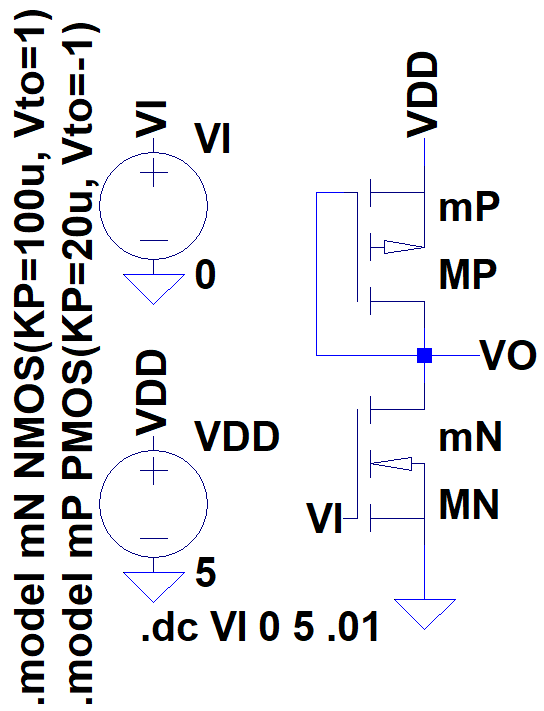
\includegraphics[width=.39\textwidth, height=\textheight, keepaspectratio=true]{ds1b}
\switchcolumn
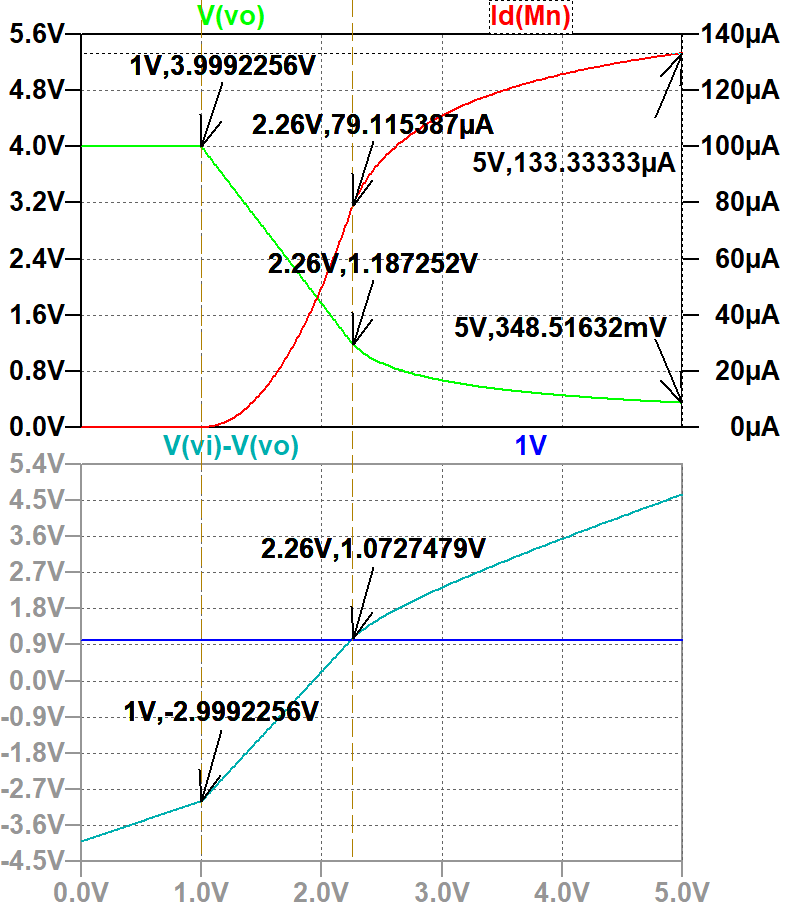
\includegraphics[width=.58\textwidth, height=\textheight, keepaspectratio=true]{ds1c}
\end{paracol}
\begin{align*}
   Err_{V_O} &= \frac{|349 - 348|}{349} = 0.28\%
\\ Err_{I_D} &= \frac{|133.3 - 133.3|}{133.3} = 0.00\%
\\ Err_{V_{It}} &= \frac{|2.236 - 2.26|}{2.236} = 1.07\%
\end{align*}
\end{center}

%\clearpage
%\columnratio{0.65}
%\begin{paracol}{2}
%\switchcolumn
%\begin{center}
%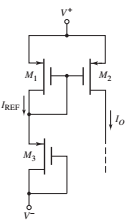
\includegraphics[width=\textwidth, height=18\baselineskip, keepaspectratio=true]{ds2}
%\end{center}
%\switchcolumn
%
%\section{Problem 16.3-9.b.1: }
%\subsection{Design}
%
%For the circuit below, find $V_{It}$, the modes of operation of the MOSFETs, $V_O$, $I_{REF}$, and the static power. Assume $V_{T1} = V_{T2} = V_{T3} = -1V$, $K_1 = 10\mu A/V^2$, $K_2 = 20\mu A/V^2$, $K_3 = 30\mu A/V^2$, $\lambda = 0$, $V_+ = 5V$, and $V_- = 0V$.
%
%\end{paracol}
%
%\clearpage
%\subsection{Validation}
%
%\begin{center}
%LTSpice Implementation
%
%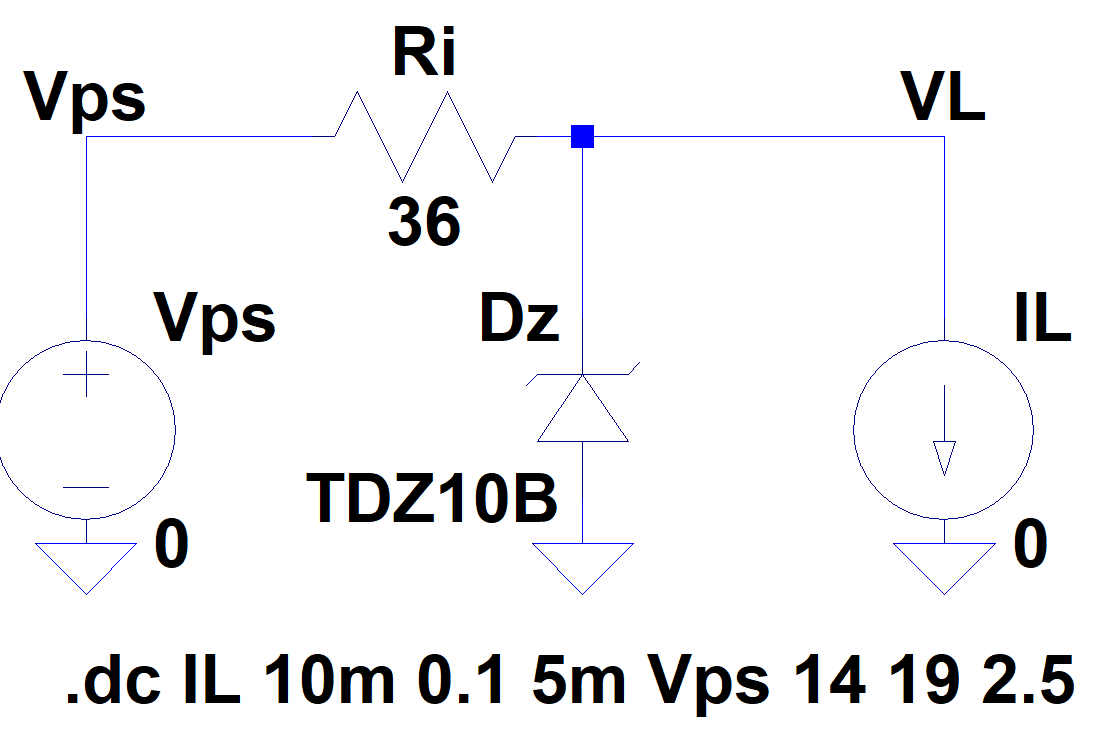
\includegraphics[width=.4\textwidth, height=\textheight, keepaspectratio=true]{ds2b}
%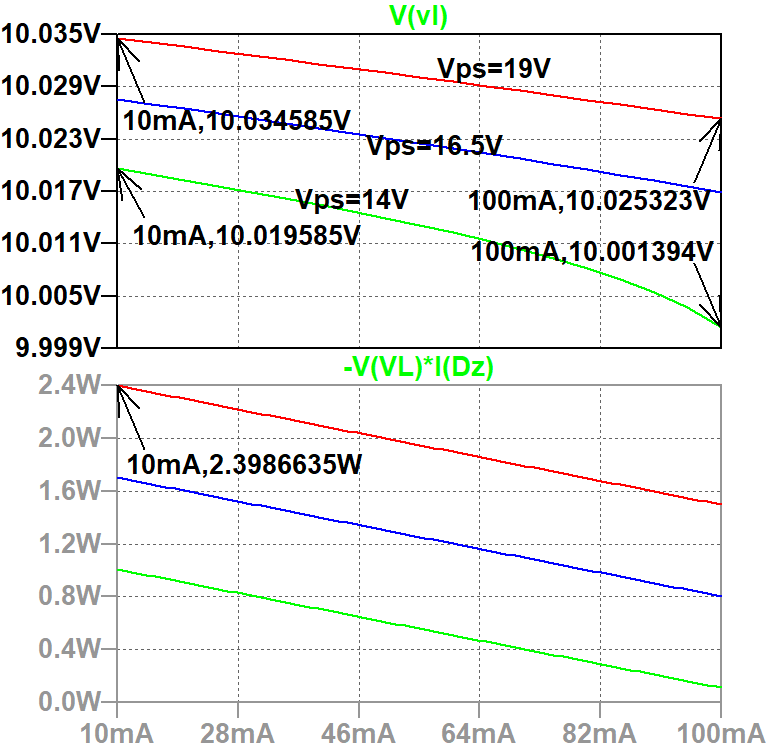
\includegraphics[width=.49\textwidth, height=\textheight, keepaspectratio=true]{ds2c}
%\end{center}

This assignment should demonstrate a basic ability to manipulate, design, and analyse enhancement load MOSFET circuits.

\textit{I have neither given nor received unauthorized assistance on this assignment.}


\end{raggedright}
\end{document}
